% ============================================================================
%  ICLR 2026 Workshop: Logical Reasoning of LLMs — 4 pages + references
%  Framing: Logical reasoning evaluation, neuro-symbolic diagnostics
%  Deadline: ~Jan 30 (suggested) — email organizers for late submission
% ============================================================================
\documentclass{article}

\usepackage[utf8]{inputenc}
\usepackage[T1]{fontenc}
\usepackage{times}
\usepackage{microtype}
\usepackage{amsmath,amssymb}
\usepackage{booktabs}
\usepackage{graphicx}
\usepackage{xcolor}
\usepackage{hyperref}
\usepackage[margin=1in]{geometry}

\definecolor{todo}{rgb}{0.8,0.1,0.1}
\newcommand{\todo}[1]{\textcolor{todo}{[TODO: #1]}}
\newcommand{\dpgap}{\textsc{D-P Gap}}
\newcommand{\da}{\textsc{DA}}
\newcommand{\pa}{\textsc{PA}}
\newcommand{\pra}{\textsc{PrA}}

\title{The Scissors Pattern: \\
Why LLMs Can Explain Logical Rules But Cannot Use Them}

\author{Anonymous}

\date{}

\begin{document}
\maketitle

% ============================================================================
\begin{abstract}
We present the \textbf{Scissors Pattern}, a diagnostic revealing
that LLMs can \emph{state} logical inference rules with near-perfect
accuracy yet \emph{fail} to apply them---with the failure growing as
rule complexity increases.
Using a 300-problem benchmark across 15 classical rules, we test
Mistral~7B and Qwen~2.5~7B (Ollama) under three conditions: Declarative (explain the
rule), Procedural (apply it), and Primed (apply it after a reminder).
Declarative Accuracy stays high ($>$0.90) across all complexity
levels, while Procedural Accuracy drops monotonically.
For Mistral~7B priming yields minimal recovery (+0.02), indicating a
\emph{binding} deficit rather than retrieval.
We release our benchmark as a diagnostic tool for the logical
reasoning community.
\end{abstract}

% ============================================================================
\section{Introduction}

Despite impressive performance on logical reasoning
benchmarks~\cite{saparov2023prontoqa,xu2024logicbench}, LLMs
consistently fail on individual inference
steps~\cite{hopp2024conditional}.
A key open question is: \emph{what kind of failure is this?}
Is the model missing the rule entirely, or does it ``know'' the rule
but fail to apply it?

We answer this by \emph{decomposing} logical reasoning accuracy into
two components inspired by Ryle's~(\citeyear{ryle1949}) distinction:
\begin{itemize}
    \item \textbf{Declarative Accuracy} (\da{}): Can the model
    correctly \emph{state} the rule?
    \item \textbf{Procedural Accuracy} (\pa{}): Can the model
    correctly \emph{apply} the rule to a novel problem?
\end{itemize}

The difference---the \textbf{Declarative-Procedural Gap}
(\dpgap{} $= \da - \pa$)---quantifies the knowing--doing
dissociation.
We discover that when rules are sorted by complexity, \da{} remains
flat while \pa{} drops, producing a distinctive \textbf{Scissors
Pattern} (Figure~\ref{fig:scissors}).

A third condition, \textbf{Primed} (\pra{}), provides the rule
explicitly before the problem.
The \textbf{Priming Effect} (\pra{} $-$ \pa{}) estimates what
fraction of the failure is due to \emph{retrieval} (the model
doesn't find the right rule) vs.\ \emph{computation} (the model
finds it but applies it incorrectly).

% ============================================================================
\section{Method}

\paragraph{Rules.}
15 classical inference rules at complexity levels 1--4
(Table~\ref{tab:rules}).

\begin{table}[t]
\centering
\small
\begin{tabular}{lc|lc}
\toprule
\textbf{Rule} & \textbf{C} & \textbf{Rule} & \textbf{C} \\
\midrule
Modus Ponens & 1 & De Morgan I & 3 \\
Double Neg. & 1 & De Morgan II & 3 \\
Modus Tollens & 2 & Biconditional & 3 \\
Hyp.\ Syll. & 2 & Absorption & 3 \\
Disj.\ Syll. & 2 & Proof by Contr. & 4 \\
Contrapositive & 2 & Constr.\ Dilemma & 4 \\
Transitivity & 2 & Material Imp. & 4 \\
Univ.\ Inst. & 2 & & \\
\bottomrule
\end{tabular}
\caption{15 inference rules with complexity (C).}
\label{tab:rules}
\end{table}

\paragraph{Problems.}
20 problems per rule (300 total). Each requires exactly one rule,
has unambiguous ground truth, and uses diverse entities to prevent
memorisation.

\paragraph{Conditions.}
(A)~\textbf{Declarative}: ``Explain [rule name].''
(B)~\textbf{Procedural}: ``Solve: [problem]'' (rule not named).
(C)~\textbf{Primed}: ``Recall [rule]: [definition]. Solve: [problem].''

\paragraph{Model.}
Mistral~7B (Ollama), temperature~0.0, JSON via prompt.

\paragraph{Scoring.}
Declarative: LLM-as-judge (3-point rubric).
Procedural/Primed: keyword matching + LLM-as-judge fallback.

% ============================================================================
\section{Results}

\paragraph{Overall.}
$\da = 0.90 \pm 0.05$, $\pa = 0.25 \pm 0.07$,
$\pra = 0.27 \pm 0.07$.
\dpgap{} $= +0.65$ (paired $t$-test: $t = 8.09$, $p < 0.001$;
Cohen's $d = 2.16$).
Priming Effect $= +0.02$.

\paragraph{The Scissors Pattern.}
Figure~\ref{fig:scissors} shows the signature result:
\da{} (blue) stays high and flat while \pa{} (red) drops from
1.00 to 0.48 with increasing complexity.

\begin{figure}[t]
\centering
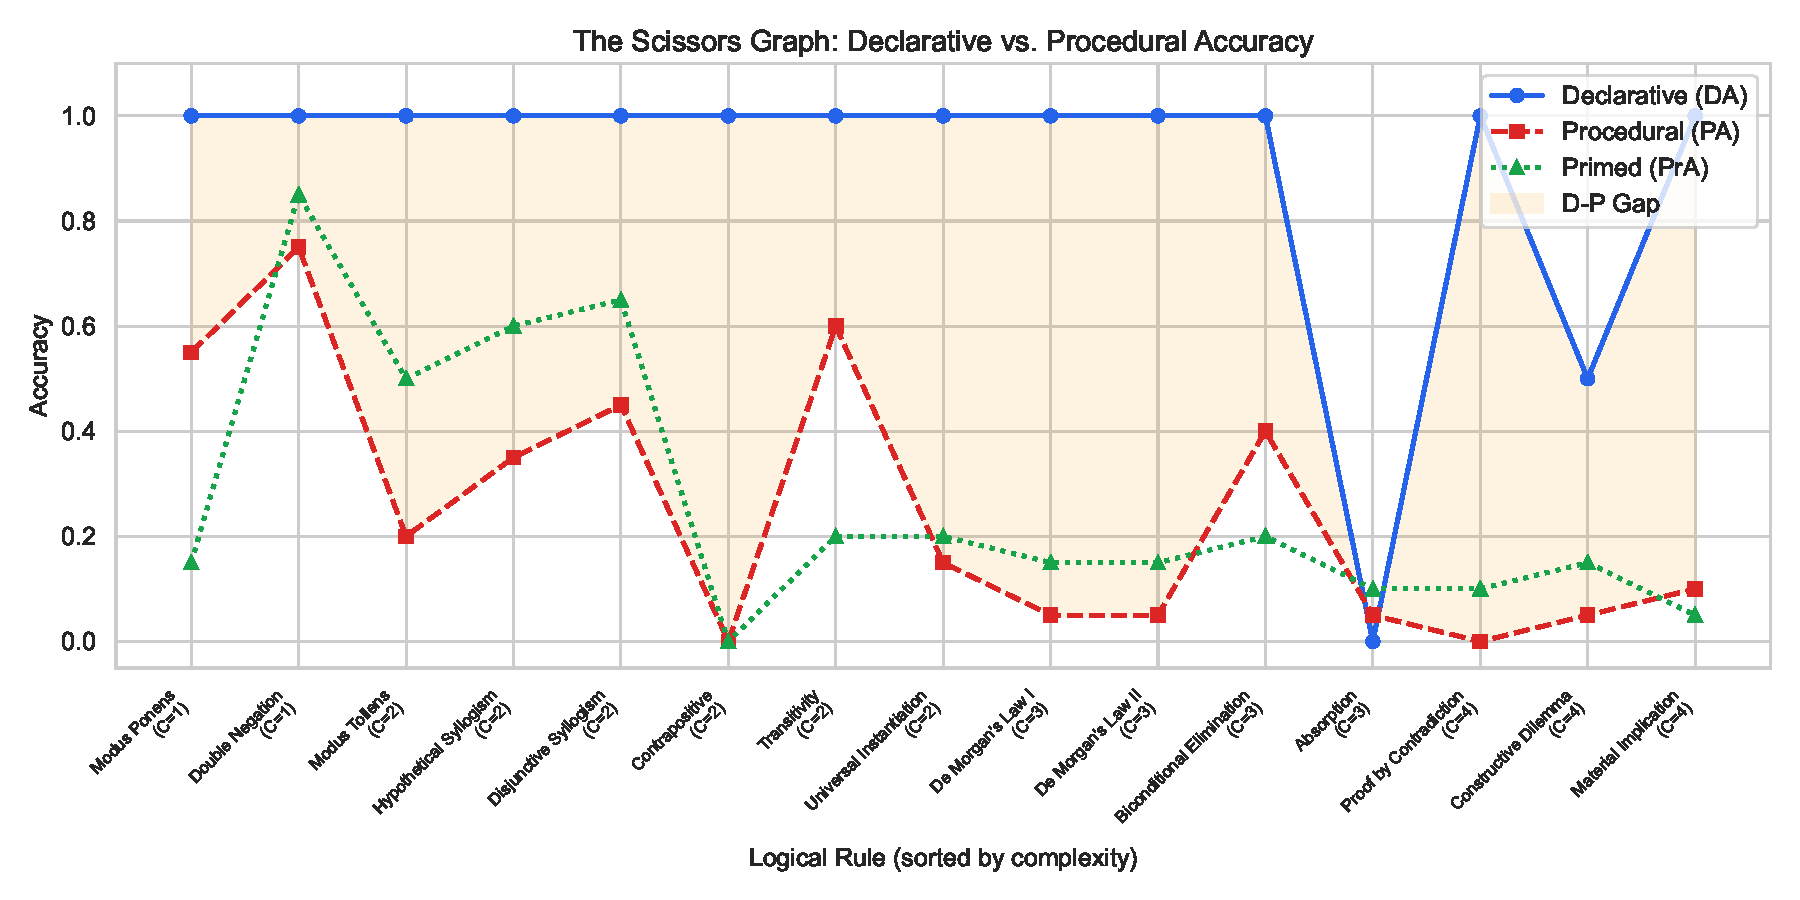
\includegraphics[width=\columnwidth]{results/scissors_graph.pdf}
\caption{The Scissors Pattern. \da{} (blue) stays flat; \pa{} (red)
drops with complexity. \pra{} (green) shows partial recovery.}
\label{fig:scissors}
\end{figure}

\paragraph{Key findings.}
\begin{enumerate}
    \item \dpgap{} is highly significant
    (paired $t$-test: $t = 8.09$, $p < 0.001$; Wilcoxon $W = 1.00$, $p = 0.001$).
    \item \dpgap{} correlates positively with complexity
    (Spearman's $\rho = 0.38$, $p = 0.17$).
    \item Priming recovers little overall (+0.02); deficit is largely binding, not retrieval.
    \item Largest gaps: Contrapositive, Proof by Contradiction (+1.00), De~Morgan I/II (+0.95), Material Implication (+0.90).
    \item Smallest gap: Absorption ($-$0.05); Double Negation (+0.25).
\end{enumerate}

% ============================================================================
\section{Analysis}

\paragraph{Retrieval vs.\ binding.}
The Priming Effect provides a natural decomposition:
\begin{align*}
\text{Retrieval deficit} &\approx \pra - \pa \\
\text{Binding deficit} &\approx \da - \pra
\end{align*}
If priming fully closes the gap (\pra{} $\approx$ \da{}), the
failure is purely retrieval.
If priming does not close the gap (\pra{} $\ll$ \da{}), there is a
residual \emph{binding} or \emph{computational} failure---the model
is given the rule but still cannot correctly instantiate it.

\paragraph{Connection to the Reversal Curse.}
The Reversal Curse~\cite{berglund2024reversal} is a
\emph{directional} asymmetry (A$\to$B $\neq$ B$\to$A).
The \dpgap{} is a \emph{modal} asymmetry
(state(rule) $\neq$ apply(rule)).
Both suggest that auto-regressive models encode knowledge in ways
that are surprisingly task-dependent.

\paragraph{Implications for benchmarking.}
Reporting a single ``logic accuracy'' score obscures the knowing--doing
gap.
We advocate for \emph{decomposed} evaluation: always report both
declarative and procedural accuracy.

\paragraph{Implications for system design.}
The Priming Effect suggests that rule-injection (via RAG or
neuro-symbolic pipelines) can partially close the gap without
fine-tuning---a practical and cheap intervention.

% ============================================================================
\section{Limitations and Future Work}

Primary results from Mistral~7B (Ollama); propositional/first-order logic
only. The \textbf{same model} was used for generation and for LLM-as-judge scoring; LLM-as-judge may introduce noise.
Future directions: multi-model comparison, temporal/modal logic,
fine-tuning interventions, mechanistic interpretability of the
binding failure.

% ============================================================================
\section{Conclusion}

We introduce the Scissors Pattern as a diagnostic for LLM logical
reasoning.
The pattern reveals that LLMs possess logical rules in a declarative
sense but cannot reliably deploy them procedurally---and this gap
widens with complexity.
Priming yields minimal recovery (+0.02) for Mistral~7B, indicating the deficit is largely binding rather than retrieval.
Our benchmark and decomposition framework are available for community
use.

\bibliography{references}
\bibliographystyle{plainnat}

\end{document}
